\documentclass[aspectratio=169,10pt]{beamer} \mode<presentation>
\usetheme[numbering=fraction]{Boadilla}
\setbeamertemplate{navigation symbols}{}

% --- Fonts & math (LuaLaTeX) ---
\usepackage{fontspec}
\usepackage{mathtools}     % load before unicode-math
\usepackage{unicode-math}
\unimathsetup{
  warnings-off = {
    mathtools-overbracket,
    mathtools-colon
  }
}

\setsansfont{TeX Gyre Heros}
\setmonofont{JetBrains Mono}
\setmathfont{Latin Modern Math}

\usepackage{bookmark}
% Examples of Beamer-native tweaks
%\setbeamertemplate{enumerate items}[default]  % numbers
%\setbeamertemplate{itemize items}[triangle]   % bullets

\setbeamertemplate{items}[ball]
\setbeamertemplate{blocks}[rounded][shadow=true]


% --- Extras ---
\usepackage{siunitx}
\usepackage{graphicx}
\usepackage{tikz}
\usetikzlibrary{arrows.meta,positioning,calc}
\usepackage{hyperref}
\hypersetup{colorlinks=true, urlcolor=blue!70!black, linkcolor=blue!60!black, pdfpagemode=FullScreen}

% ---- Graphics path
\graphicspath{{figs/}}

% ---- Title info ----
\title{NVH, a walk down memory lane}
\subtitle{by an old applied mathematician}
\author{H\aa vard Vold}
\institute{Vold LLC}
\date{October 8-10, 2025}

% ---- Handy macros (examples) ----
\newcommand{\R}{\mathbb{R}}
\DeclareMathOperator*{\argmin}{arg\,min}

\begin{document}

% ===== Title slide =====
\maketitle

% ===== Outline =====
\section[Outline]{}
% \frame{\frametitle{Outline} \tableofcontents}
\frame{\frametitle{Outline} \tableofcontents}

\AtBeginSection[] {
  \begin{frame}{Next topic}
    \tableofcontents[currentsection]
  \end{frame}
}

% ===== Section 3 =====
\section{Places I have been}
\begin{frame}[t]{Places I have been}
  \begin{itemize}[<+->]
    \item Institute of Mathematics, University of Oslo
    \item Institut f\"u{}r Statik und Dynamik (ISD), University of Stuttgart
    \item Structural Dynamics Research Corporation, Cincinnati, Ohio
    \item SDRL, University of Cincinnati, Ohio
    \item ATA Engineering, San Diego, California
    \item Vold LLC, back on the farm in M\aa{}ndalen, Norway
  \end{itemize}
\end{frame}

\section{Modal Testing}

\subsection{Parameter Estimation}

\begin{frame}[t]{Prony Algorithm}
  Baron Gaspard Clair François Marie Riche de Prony, 1755 -- 1839
  \vspace{8mm}
  \begin{itemize}[<+->]
    \item Prony devised in 1795 an algorithm to estimate an expansion of exponentials to a measured function.
    \item Spitznogle of the US Navy used the same method, but with complex exponentials to investigate radar signals and to account for oscillation and damping. The year was 1955.
    \item Around 1980 the idea was introduced as the \it{complex exponential} method to experimental modal analysis.
  \end{itemize} 
  \vspace{5mm}
  \uncover<+->{
  \begin{block}{The paper that started it all}
  \it{Essai expérimental et analytique sur les lois de la dilabilité des
fluides élastiques, et sur celles de la force expansive de la vapeur de l’eau
et de la vapeur de l’alkool, à différentes températures}, Journal de l’École
polytechnique 2 (1795), 24 – 77.
\end{block}
}
\end{frame}

\begin{frame}{Polyreference Time Domain}
  \begin{block}{The AHA! moments}
    \begin{itemize}[<+->]
    \item It was observed that a least square average was possible with the Prony method by using a set of unit impulse response functions for sharper parameter estimates    
    \item I noticed that the scalar equations still made sense when looking at vector time histories of free decay
    \item Yes, we now had to pay homage to non commutation and transpose and complex conjugate when required. Same formulae, but written in \bf{boldfaced type}
    \item Instead of finding zeros of a scalar polynomial we now determine the eigenstructure of a high order matrix polynomial
  \end{itemize}
\end{block}

\uncover<+->{
  \begin{block}{Polyreference}
   \begin{itemize}
     \item Can now resolve repeated roots with full subspace of eigenvectors
     \item We're saving space by using the reciprocity theorem and looking at unit impulse responses for the excitation freedoms only
     \item Perfect companion for simultaneous incoherent multishaker excitation
   \end{itemize} 
  \end{block}
}
\end{frame}


\subsection{Multiple Exciter Locations}
\begin{frame}[t]{Simultaneous Partially Incoherent Excitation}
  \begin{block}{Features}
    \begin{itemize}[<+->]
      \item Even distribution of energy across structure
      \item Excite more modes
      \item Consistent response relative to all exciter locations
      \item Faster!!
    \end{itemize}
  \end{block}
  \begin{block}{Gotchas}
    \begin{itemize}[<+->]
      \item More instrumentation
      \item Nonlinear structures will not reach limit cycle
      \item Symmetric excitation on symmetric structures defeats purpose
      \item Multiple coherence is often too optimistic
      \item $H_2$ FRF estimator unavailable; $H_1$ and $H_v$ work as expected
    \end{itemize}
  \end{block}
\end{frame}

\subsection{Structural Modification using FRF}
\begin{frame}[t]{SMURF by Lagrange Multipliers}
  \begin{block}{History}
    \begin{itemize}[<+->]
      \item Structural modification for tuning dampers was popular in the late seventies
      \item At SDRC we decided to try to enforce linear constraints on experimental FRF matrices
      \item In 1983 we published a simple solution with Lagrange multipliers and had some success
      \item But we stopped at simple problems because we ran into problems since we did not have rotational measurements
    \end{itemize}
  \end{block}
  \begin{block}{Now, however}
    \begin{itemize}[<+->]
      \item Around 2010 in M\"u{}nchen and Delft, researchers picked this up again and added \it{virtual degrees of freedom}
      \item These virtual freedeoms were constructed as linear functions of measured freedoms and could e.g., give reasonable estimates for the rotations that we could not measure and therefore gave up
      \item This has given a totally new life to blocked forces and dynamic substructuring at high frequencies
    \end{itemize}
  \end{block}
\end{frame}

\section{Shuttle Orbiter Modal Test 1983}

\begin{frame}
  \frametitle{First Large Scale Multishaker Modal Test}
  \begin{figure}
    \centering
    \includegraphics[width=0.65\linewidth,height=7cm]{SDRC-shuttle-1983}
  \end{figure}
    \center{Shuttle GVT at Edwards AFB, 1983}
\end{frame}

\begin{frame}
  \frametitle{Claiming the Shuttle Orbiter Vehicle for Norway, 1983}
  \begin{figure}
    \centering
    \includegraphics[width=0.65\linewidth,height=7cm]{Shuttle-1983}
  \end{figure}
    \center{Screwed up the paperwork and had to leave it at Edwards AFB}
\end{frame}

%adding in the old material
\section{Vold-Kalman Filter}
\begin{frame}[t]{Tracking Unsteady Sinusoids inspired by Bucy and Kalman}
 \begin{block}{History}
   \begin{itemize}[<+->]
    \item[ 1993] Vold and Leuridan published a paper on the time domain extraction of orders with phase and amplitude information from rotating systems with rapidly changing rotary speeds
    \item[ 1995] Vold developed a second generation algorithm that could resolve close and crossing orders from systems with multiple independent exciting sources
  \end{itemize}
 \end{block} 
 \uncover<+->{
\begin{block}{The good and the bad}
  \begin{itemize}[<+->]
    \item No phase bias since the formulations are symmetric in time
    \item Original signal could be edited for sound quality studies since no phase bias
    \item Same time resolution as the original time histories
    \item Setting the bandwidth was alchemy until 2004 when Jiri Tuma found an analytical formula
    \item Compute time used to be atrocious, but is now much more reasonable
 \end{itemize} 
\end{block}
 }
\end{frame}

 
\section{Spacecraft Cabin Ventilation Fan in NASA Glenn Acoustical Test Laboratory}
\frame{\frametitle{Spacecraft Cabin Ventilation Fan in Acoustical Test Lab}
  Microphone array traverses 168\,inches at 1\,inch/second continuously.\\
  Fan runs at 12,000\,RPM. 9 blades in rotor.
  \begin{columns}[t]
    \column{0.3\textwidth}
    \begin{figure}
      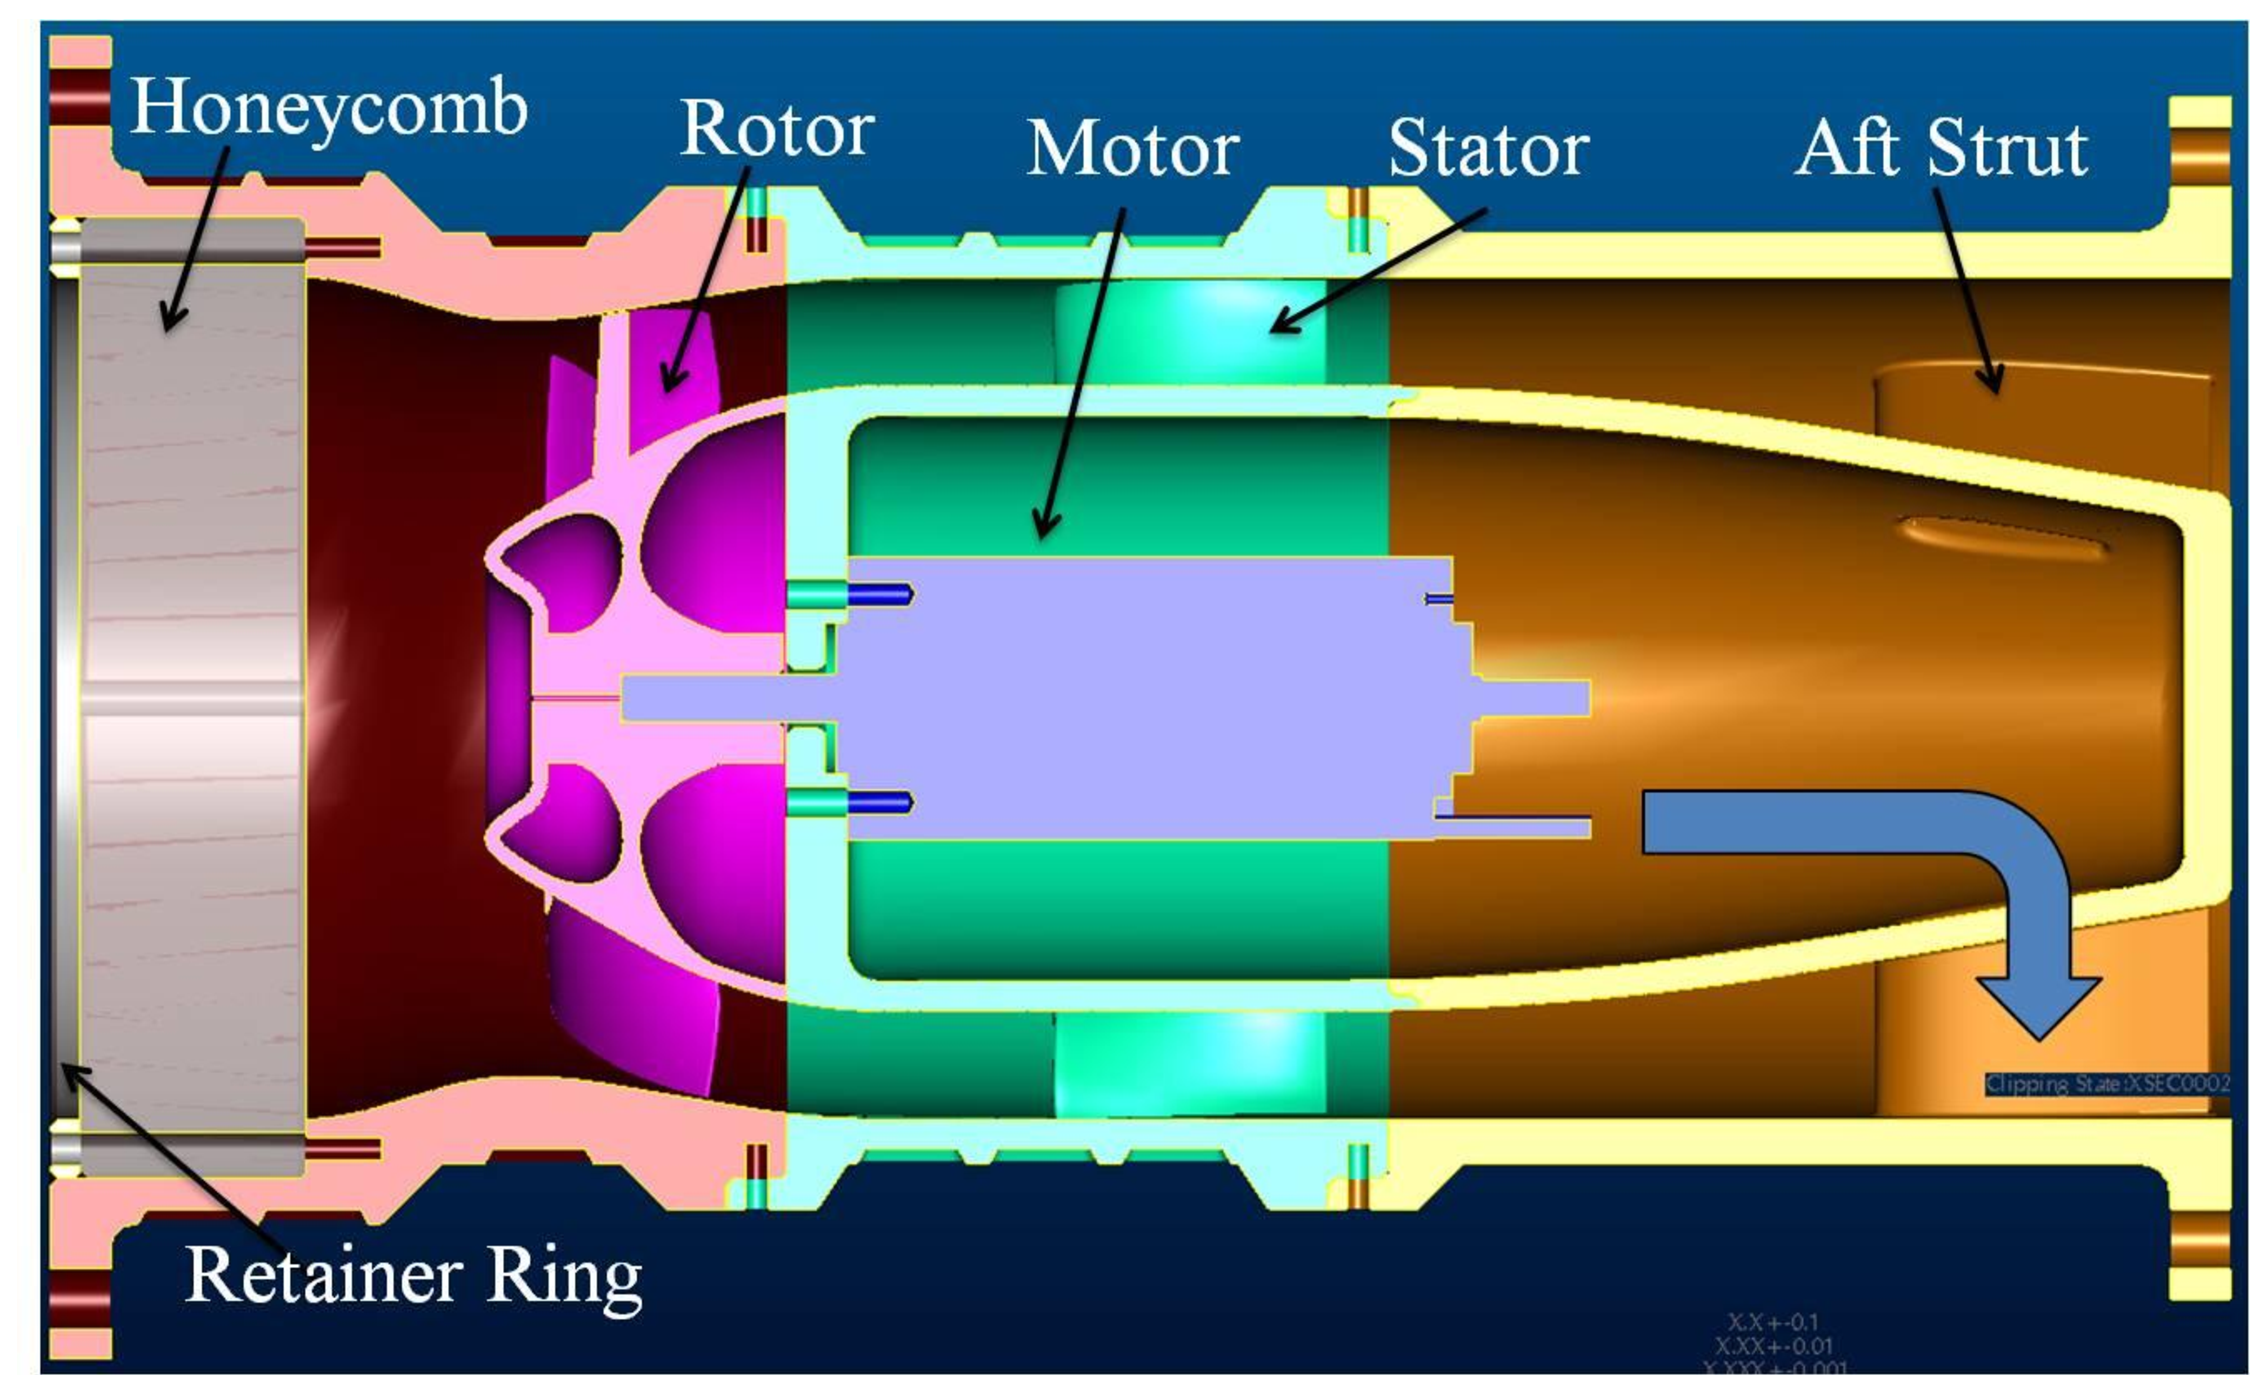
\includegraphics[width=3cm]{Spacefan03262012}
    \end{figure}
    \begin{figure}
      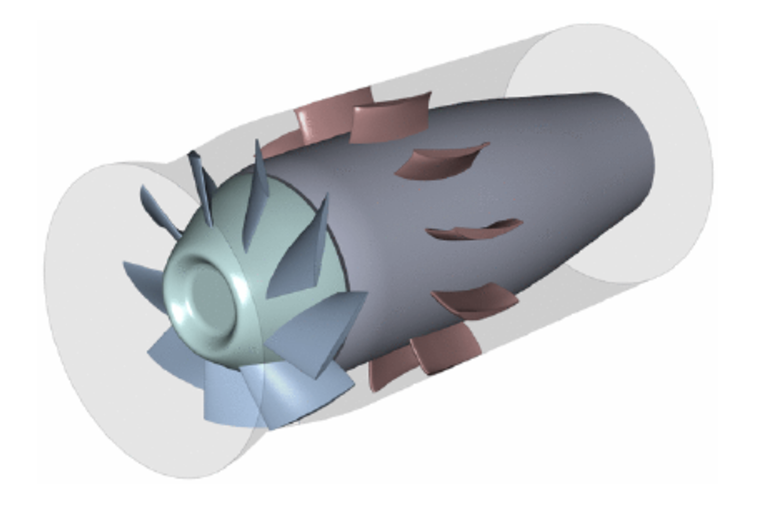
\includegraphics[width=3cm,trim=0 40 0 0]{VentFanAeroDesign}
    \end{figure}
    Fan size 9 by 4\,inches \column{0.7\textwidth}
    \begin{figure}
      \includegraphics[width=7cm,trim=0 20 0 80]{2011_04416_300}
    \end{figure}
  \end{columns}
}

\frame{\frametitle{POD of 4 Stationary Microphones (principal spectra)} 
  Blade passes 1, 2
  and 3 at 1.8\,kHz, 3.6\,kHz and 5.4\,kHz generate \emph{self-coherent} sound
  fields. Several \emph{mutually incoherent} broadband sound fields in each frequency
  band.
  \begin{figure}
    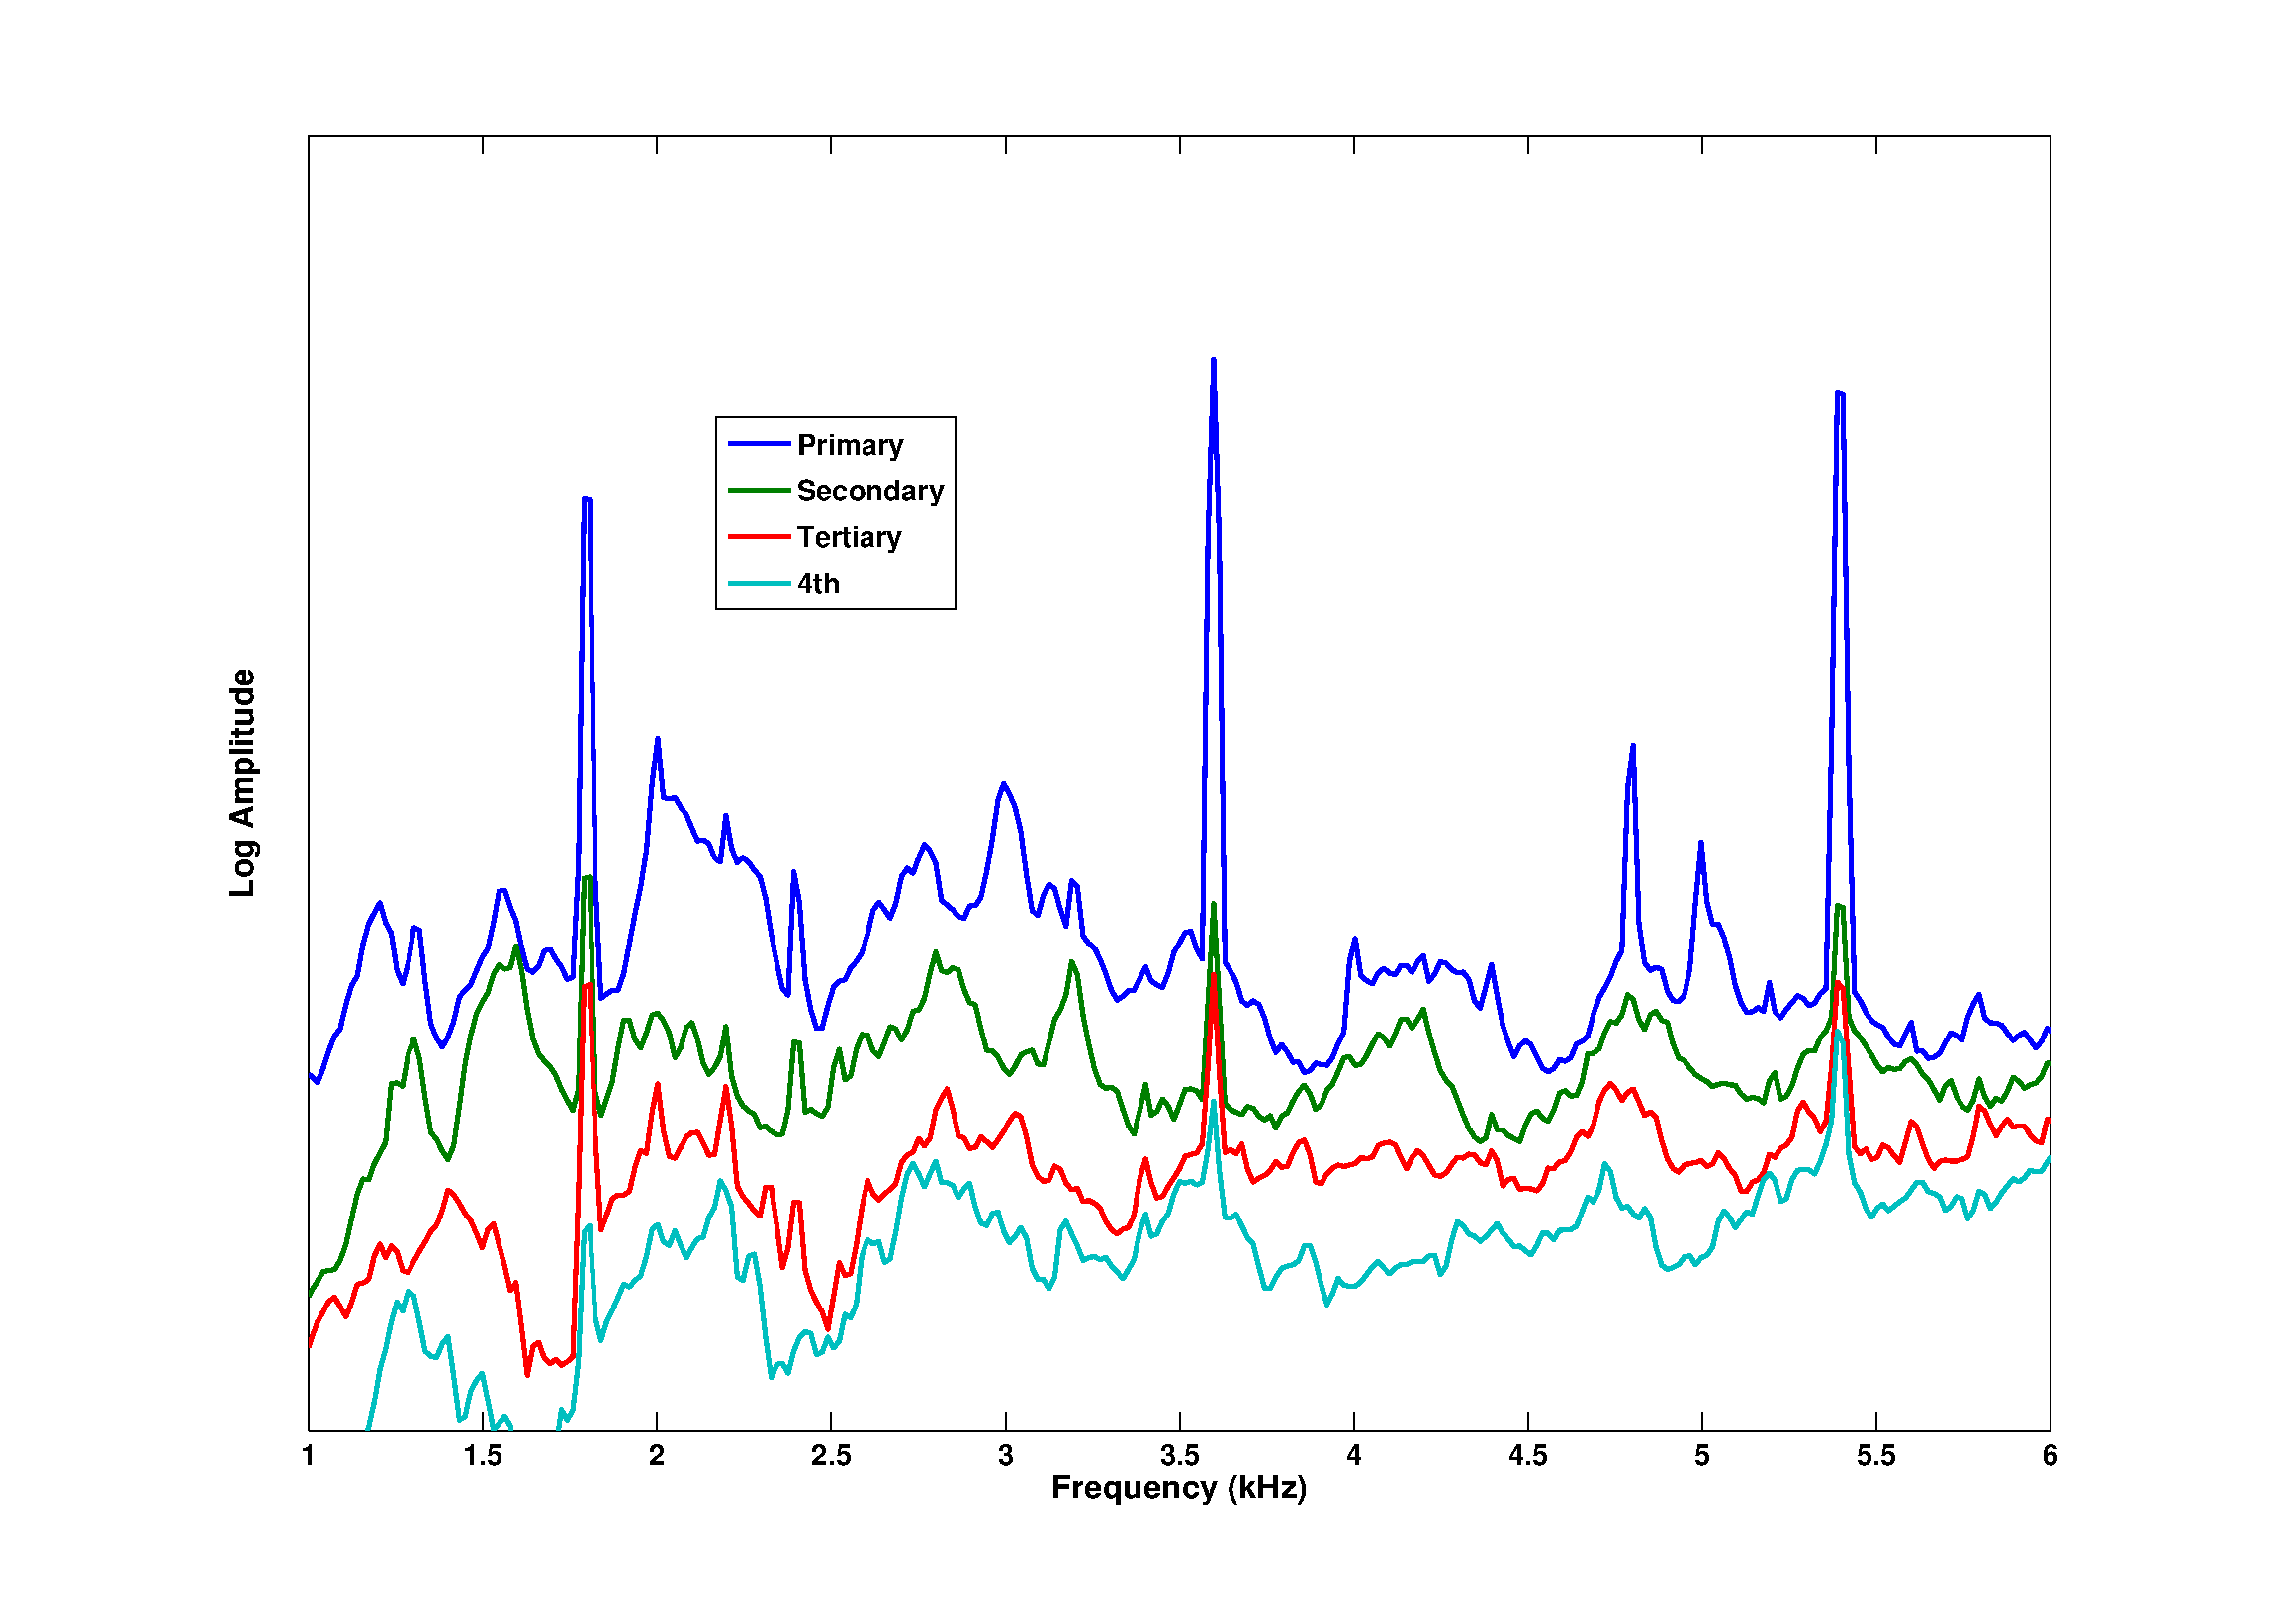
\includegraphics[width=10cm,trim=0 25 0 25]{evals}
  \end{figure}
}

\frame{\frametitle{Wold Decomposition of Center Traversing Microphone} 
  Time histories of
  sinusoids and broadband noise as function of traverse distance.  The exhaust is to the
  right in the figure. \qquad \qquad \raisebox{-2ex} {\Huge $\Longrightarrow$}
  \only<1>{
    \begin{figure}
      \includegraphics[width=10cm,height=7cm,trim=0 0 0 15]{pc1s2decomp_total_600}
    \end{figure}} \only<2>{
    \begin{figure}
      \includegraphics[width=10cm,height=7cm,trim=0 0 0 15]{pc1s2decomp_broad_600}
    \end{figure}} \only<3->{
    \begin{figure}
      \includegraphics[width=10cm,height=7cm,trim=0 0 0 15]{pc1s2decomp_harm_600}
    \end{figure}} }

\frame{\frametitle{Real Part of Bladepass 2 at Center Traversing Microphone}
  \textbf{\color{blue}{Continuous scan}} compared with \textbf{\color{red}{Fixed index
      (start--stop) with 3\,inch spacing}}. Note spatial aliasing; acoustic wavelength is
  3.7\,inches at 3.6\,kHz.  The exhaust is to the right in the figure. 
  \qquad \qquad \raisebox{-2ex} {\Huge $\Longrightarrow$}
  \begin{figure}
    \includegraphics[width=10cm,height=6.5cm,trim=0 0 0 15]{BP2Linescan}
  \end{figure}
}

\frame{\frametitle{Fourier Acoustics Reconstruction of BP 2 Sound Field}
  \begin{columns}[T]
    \column{0.6\paperwidth}
    \begin{figure}
      \includegraphics[width=9cm,trim=40 0 0 75]{FanWorkSheet.pdf}
    \end{figure}
    \column{0.4\textwidth} \alert<1>{Continuous scan eliminates spatial aliasing at higher
      frequencies, allowing for the
      techniques of \emph{acoustic holography} to be used. \\
      Axisymmetry is assumed.} \\
    \uncover<2>{\alert<2>{Resolution at source limited by acoustic wavelength;
        \emph{evanescent} waves have died before they reach the microphone.}}
  \end{columns}
}

\frame{\frametitle{Fourier Acoustics 1200\,Hz Broadband Sound Fields}
  \begin{columns}[T]
    \column{0.5\textwidth}
    \vspace{-0.7em}
   \center{Primary $6^{th}$ octave field\\ \alert<1>{Antisymmetric}}
    \begin{figure}
      \includegraphics[width=6cm,height=5cm,angle=90]{1200F1}
    \end{figure}
    \column{0.5\textwidth}
    \vspace{-0.7em}
    \center{Secondary $6^{th}$ octave field\\ \alert<2>{Symmetric}}
    \begin{figure}
      \includegraphics[width=6cm,height=5cm,angle=90]{1200F2}
    \end{figure}
  \end{columns}
  \center{Amplitudes scaled for graphics presentation}
}

\section{Dual Open Rotor in NASA Glenn 9x15 Wind Tunnel}
\frame{\frametitle{Dual Open Rotor in NASA Glenn 9x15 Wind Tunnel} 
  Two counter-rotating
  rotors\uncover<2->{, \color{red}{loosely coupled through control system}}
  \begin{columns}
    \column{0.45\textwidth}<1->
    \begin{figure}
      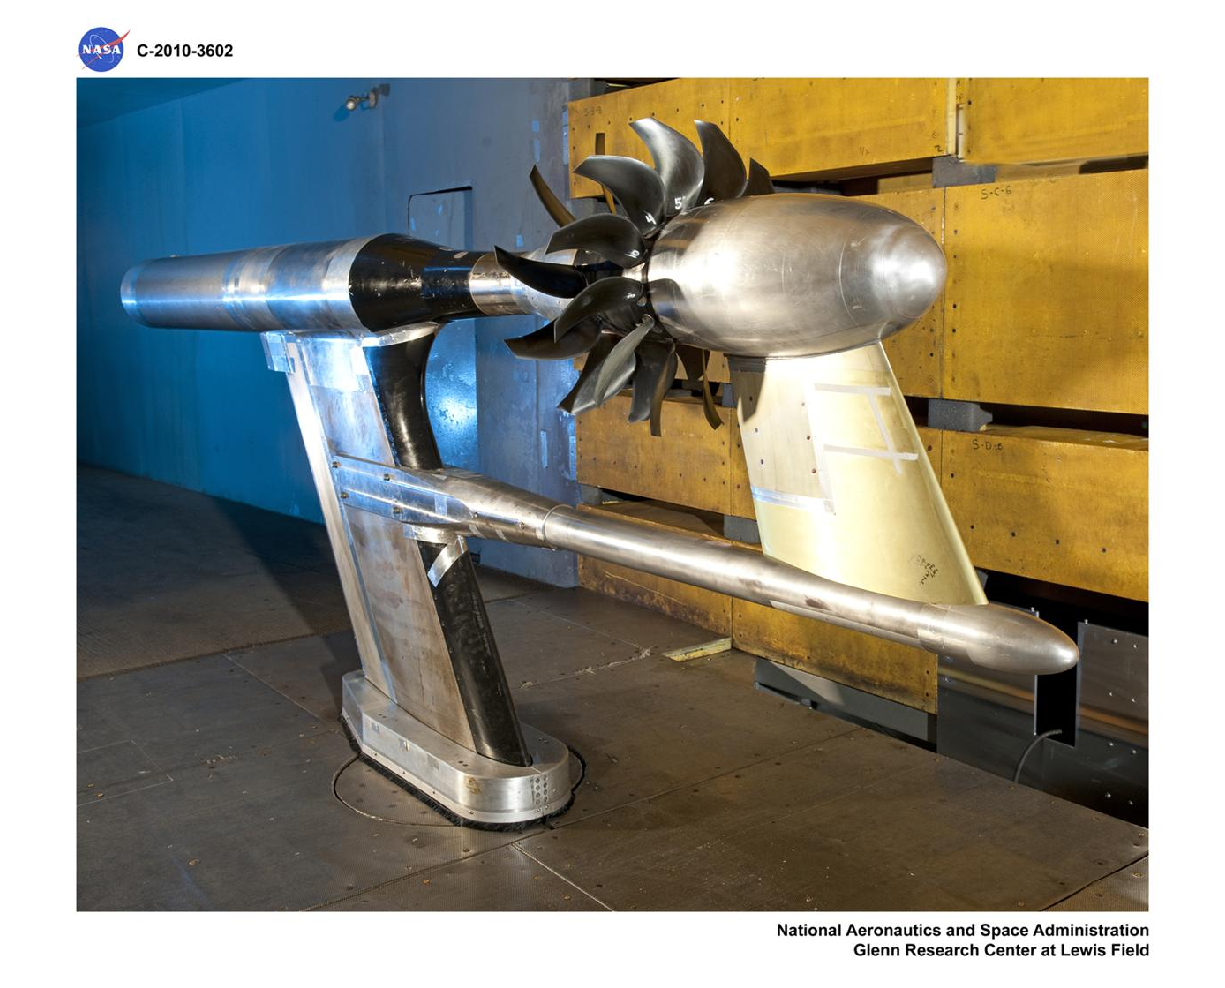
\includegraphics[height=5cm]{2010_03602_150_Small}
    \end{figure}
    \center{\color{black}{Back to the future\\Hardware anno 1988}} 
    \column{0.55\textwidth}<2->
    \vspace{1cm}
    \begin{figure}
      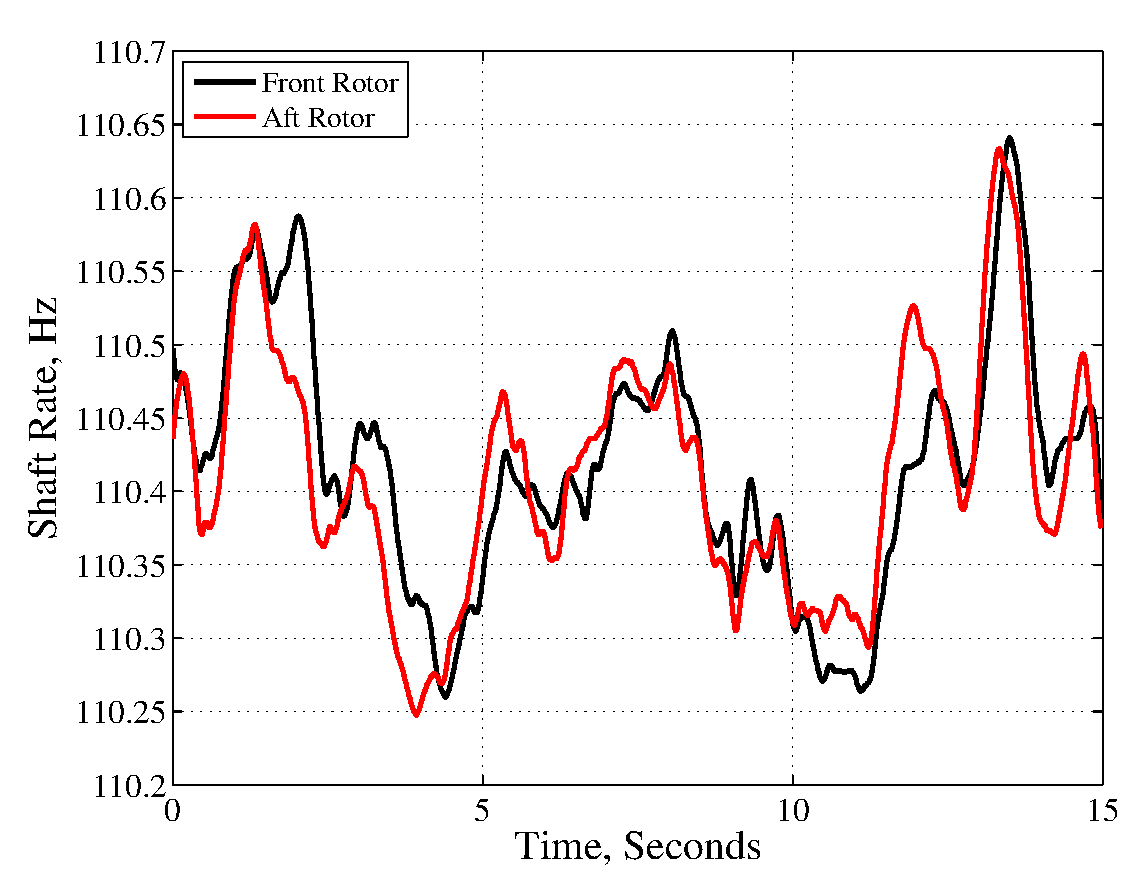
\includegraphics[width=5cm,height=4cm]{RPM_Example_472_8}
    \end{figure}
    \center{\alert<2->{Time histories of rotor speeds}}
  \end{columns}
}

\frame{\frametitle{Removing Tones with the Vold-Kalman Filter} \only<1>{ \center{PSD of
      total signal\\Tones and broadband noise}
    \begin{figure}
      \includegraphics[width=10cm]{RDG_446_VK_Compare_total}
    \end{figure}} \only<2>{ \center{PSD of signal with tones removed
      shaft--by--shaft\\Interaction tones cause trouble}
    \begin{figure}
      \includegraphics[width=10cm]{RDG_446_VK_Compare_serial}
    \end{figure}} \only<3->{ \center{PSD of signal with tones removed
      simultaneously\\Interaction tones behave}
    \begin{figure}
      \includegraphics[width=10cm]{RDG_446_VK_Compare_parallel}
    \end{figure}} }

\begin{frame}
\frametitle{Fourier Acoustics Sound Fields --- Tones 40 and 48}
{ Continuous scan over 6.6\,meters, 600 second scan\\
Traversing microphone 1.52\,meters from centerline\\
\raisebox{-1ex} {\Huge $\Longleftarrow$} Mach 0.2 mean flow}
\vspace{-1em}
  \begin{columns}[T]
    \column{0.5\textwidth}
   \center{Order 40 Rear}
    \vspace{-1em}
    \begin{figure}
      \includegraphics[width=6cm,height=5.5cm]{O40S2H}
    \end{figure}
       \column{0.5\textwidth}
    \center{Order 48 Front}
    \vspace{-1em}
    \begin{figure}
      \includegraphics[width=6cm,height=5.5cm]{O48S1H}
    \end{figure}
  \end{columns}
  \center{Amplitudes scaled for graphics presentation}
\end{frame}

\frame{\frametitle{Fourier Acoustics Sound Fields --- Tones 10 and 12}
{Continuous scan over 6.6\,meters, 600 second scan\\
Traversing microphone 1.52\,meters from centerline\\
\raisebox{-1ex} {\Huge $\Longleftarrow$} Mach 0.2 mean flow}
\vspace{-1em}
  \begin{columns}[T]
    \column{0.5\textwidth}
   \center{Order 10 --- Aft Rotor}
    \vspace{-1em}
    \begin{figure}
      \includegraphics[width=6cm,height=5.5cm]{O10S2H}
    \end{figure}
    \column{0.5\textwidth}
    \center{Order 12 --- Front Rotor}
    \vspace{-1em}
 \begin{figure}
      \includegraphics[width=6cm,height=5.5cm]{O12S1H}
    \end{figure}
  \end{columns}
  \center{Amplitudes scaled for graphics presentation}
}

 % end of adding in the old material
% ===== References (biblatex optional) =====
% For a short deck you can hand-write citations; for larger talks use biblatex:
% \begin{frame}[allowframebreaks]{References}
%   \tiny
%   \printbibliography
% \end{frame}

% ===== Closing =====
\section{Conclusion}

\begin{frame}{Takeaways}
\begin{enumerate}
  \item Key result 1
  \item Key result 2
  \item Code / repo / contact: \href{mailto:hvold@vold.com}{hvold@vold.com}
\end{enumerate}
\end{frame}

\begin{frame}[standout]
Questions?
\end{frame}

\end{document}

